\documentclass{llncs}
%
\usepackage{graphicx}
\title{Accessible EPUB : Creating an EPUB IDE to create accessible documents}
\author{Sachin Rajgopal\inst{1}, Thorsten Schwarz\inst{1}, Rainer Stiefelhagen\inst{1}}

\institute{Karlsruhe Institute of Technology}

\date{}

\begin{document}

\maketitle

\begin{abstract}
	This extended abstract first discusses the E-book format EPUB as electronic format and its potential benefits for people with accessibility requirements over established documents formats like PDF and word documents. Furthermore, a new EPUB editor called Accessible EPUB is introduced, which will allow teachers to create accessible EPUBs with limited coding ability for students with accessibility requirements. 
\end{abstract}

\section{Introduction}
Over the last several years, accessibility is becoming a word with ever increasing importance. Several nations have passed regulatory acts which guarantee equal treatment between all people and that documents have to be accessible for everyone.
\cite{webaim}

Currently, the dominant format for electronic documents are PDFs (Portable Document Format, extension .pdf) and word documents(extension .doc, .docx, .odt). While PDF/UA (PDF/Universal Accessibility) has done much in terms of accessibility, there are still some shortcomings. First of all both formats have a predefined page size. While this is useful when printing documents, a computer screen can rarely display all contents of the document.\cite{EPUBzone} The font size is also set. Visually impaired people will have difficulty reading and moving the page simultaneously.
On the other hand, this means that an electronic document format with no set document size, containing semantic and structure information and a set reading order would be better suited to meet the demands of accessibility.\cite{EPUBzone}

\subsection{EPUB}
EPUB stands for electronic publication and is a format primarily used for books in an electronic format (E-book). The EPUB format was created by the International Digital Publishing Forum (IDPF) and the current version is 3.1, which is a minor update to EPUB 3.\cite{EPUBspecs} EPUB uses XML based formats like XHTML, and thus also uses the accessibility standards and guidelines already established in many nations. The Web Content Accessibility Guidelines (WCAG) can be followed to create accessible EPUB documents.\cite{WCAG} This was done as reading systems can have different screen sizes and the EPUB content can therefore be reflowable. Font type, size and color can also be changed. Visually impaired people could therefore adjust the document to their preferences. The EPUB3 specification also contains guidelines for accessibility so these features are built in and not an afterthought.\cite{EPUB3bp}

The EPUB working group has also made some important changes from EPUB 2 to EPUB 3  to make it more accessible. Equations can now be displayed in MathML, there is better navigation and more support for Cascading Style Sheets (CSS). However, not all of these changes are supported yet by many EPUB reading programs and devices.\cite{EPUB30changes} DAISY (Digital Accessible Information System), the audio substitute for print media for the blind, has now been integrated into EPUB 3.\cite{daisyAccessibility}

\subsection{EPUB Creation Process}
An EPUB file is actually just a ZIP file but renamed.\cite{WhatIsEpub3} Once the file extension is changed and and file contents are extracted, the individual files, like XHTML and image files, can be opened. So creating an EPUB can be described briefly in three steps: create the content documents like XHTML and SVG, then create the package document  called package.opf and finally zip up the file with meta-data.
The package document has five sections which describe how the EPUB document is structured.\cite{EPUB3bp}

\subsection{Existing EPUB editors}
There are many EPUB creators such as Adobe InDesign. Adobe InDesign is suitable for publishers, but it does not have inbuilt MathML support, and it is a commercial program which might not be affordable for teachers.

%\begin{figure}
%	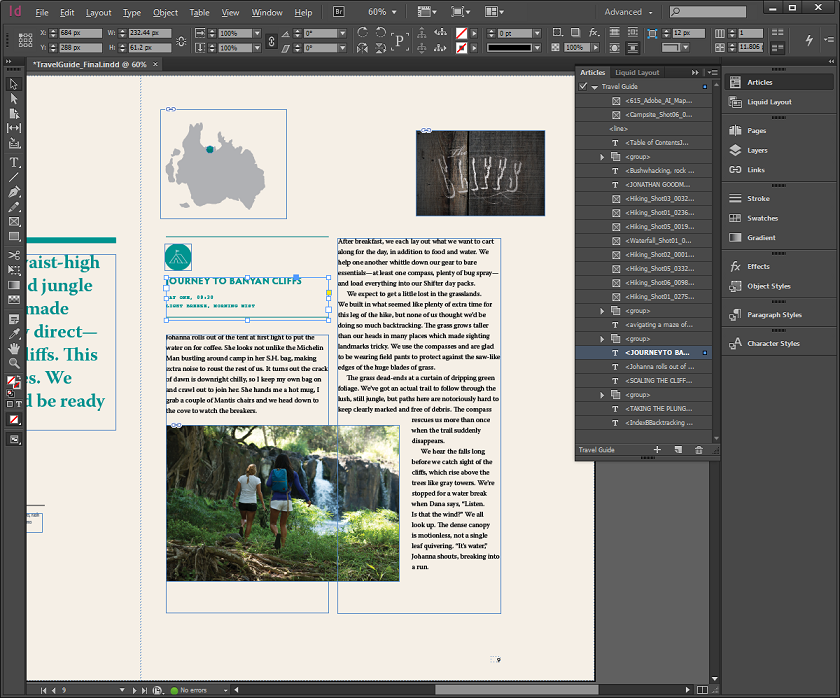
\includegraphics[height=100mm]{AdobeInDesign.png}
%	\caption{Adobe InDesign}
%\end{figure}

A word document can also be converted to an EPUB file, but there may be some adjustments which have to be made later with an EPUB editor, which usually involves coding. 
Some EPUB editors are purely WYSIWYG (What You See Is What You Get), but important features like mathematical equations and semantic information tend to be missing. EPUB editors where the program code has to be edited is limited to people with coding experience.

Sigil is a WYSIWYG, open source EPUB editor.\cite{Sigil} It has many features, but important features for accessibility, like text alternatives for images, can only be added with coding.
Lastly, many of the editors are not accessible by visually impaired blind people. 


\section{Specfications of Accessible EPUB}

\subsection{EPUB switching mechanism}

From the introduction it is apparent that while EPUBs are a promising format, the lack of easily usable editors means that not everyone can create accessible EPUBS.

Therefore the main goal of this article to describe a program called Accessible EPUB, which allows people, predominantly teachers, to create an EPUB which can be used by blind, visually impaired and regularly sighted people. By changing the CSS with a click for each target group, the EPUB will be change its content to match the target group's requirements. 

%\begin{figure}
%	\centerline{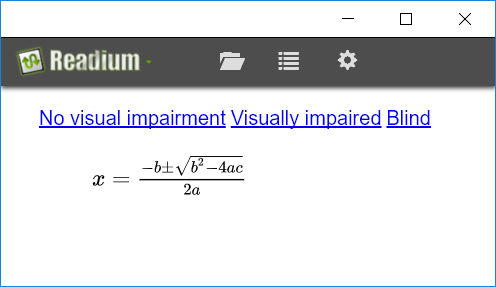
\includegraphics{EquationNormal.png}}
%\end{figure}

%\begin{figure}
%	\centerline{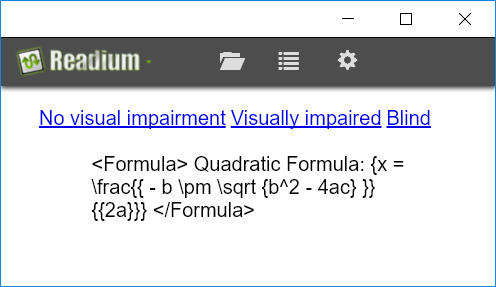
\includegraphics{EquationLatex.png}}
%\end{figure}

\begin{figure}
	\centering
	\begin{minipage}{0.45\textwidth}
		\centering
			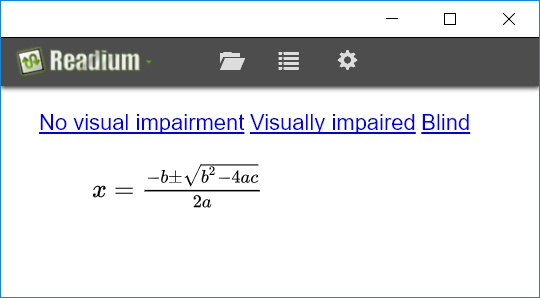
\includegraphics[width=58mm]{EquationNormal2.png} 
		\caption{Quadratic formula shown in 'No visual impairment' mode}
	\end{minipage}\hfill
	\begin{minipage}{0.45\textwidth}
		\centering
			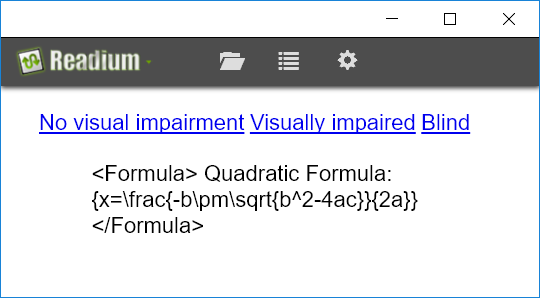
\includegraphics[width=58mm]{EquationLatex2.png} 
		\caption{Quadratic formula shown as LaTeX code in 'Blind' mode}
	\end{minipage}

\end{figure}


For example, the text alternatives for mathematical equations and images should be displayed automatically if the blind version is selected.\cite{EPUB3bp} The switching mechanism can done with either JavaScript or CSS. While using JavaScript is easier to do, not all reading devices support JavaScript nor does the EPUB specification demand that it is supported. \cite{EPUB3bp} The CSS version is much more limited as the whole content has to inserted into a single XHTML file, and CSS selectors are not supported widely yet, but CSS support is in the EPUB specification.

\subsection{Accessible EPUB}
Accessible EPUB will be a WYSIWYG program written in C\# (.NET) and will be for creating accessible EPUB documents with the switching mechanism. The document creation process should be as simple and as straight forward as possible so that people with limited experience with computers can still use the program. A primary target group is teachers with students who have a need for accessible documents.

Some of the main features of Accessible EPUB will be:

\begin{itemize}
	\item Creating an EPUB with the switching mechanism without coding it in
	\item An equation editor which accepts LaTeX as input and inserts the MathML equivalent, SVG image and the alternative text of the equation
	\item Ability to insert images with title, caption and alternative text
	\item Ability to insert tables
	\item Mark up sections using the HTML styles (h1, h2, p, etc.)
\end{itemize}



\begin{figure}
	\centering
	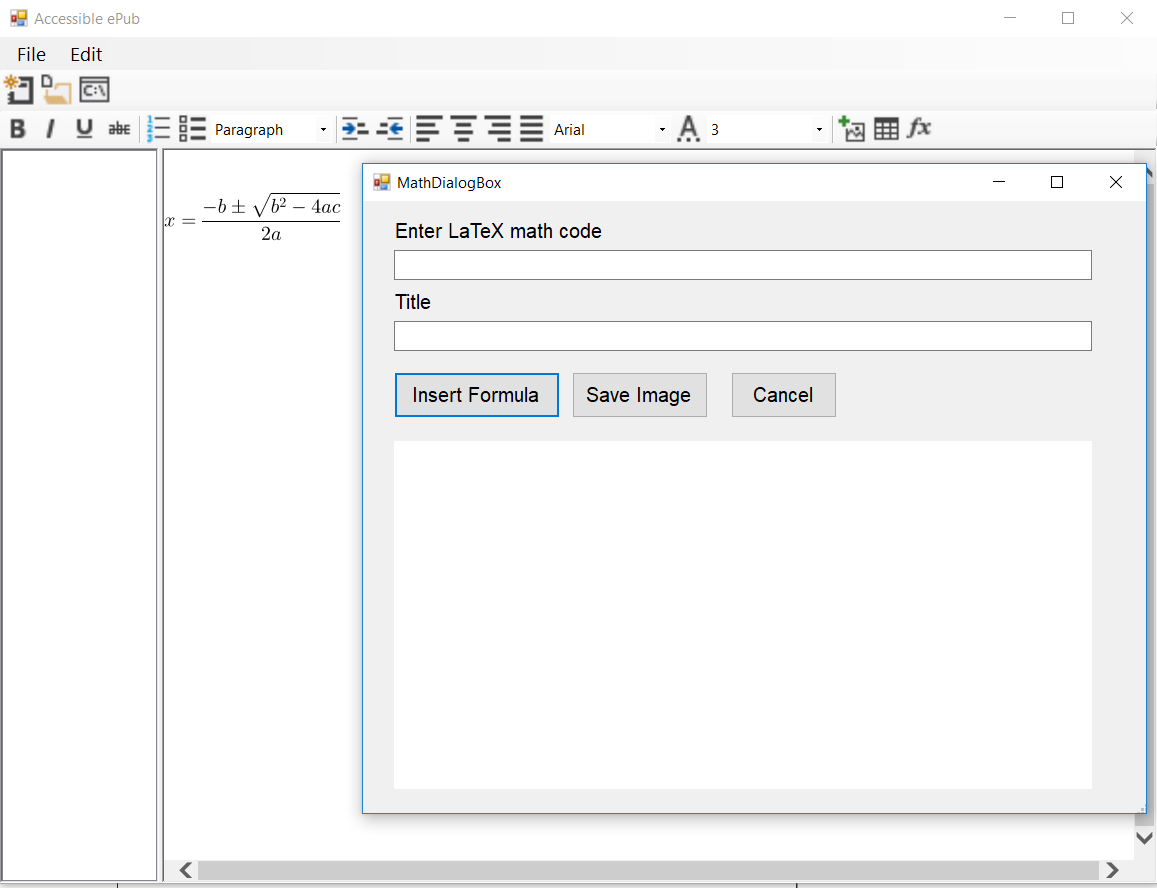
\includegraphics[height=80mm]{AccessibleEPUBequation.png}
	\caption{Accessible EPUB equation editor}
\end{figure}

\section{Outlook}
Accessible EPUB is a bachelor thesis project and is supposed to be finished by the end of March. In the final paper the project will be presented in a complete form and the results of a evaluation with student tutors and teachers will also be presented here. 

\bibliography{Accessible_EPUB}
\bibliographystyle{splncs}



\end{document}